\chapter{Proceso de Construcción y Evaluación del \textit{Pipeline}} \label{cap:metodologia}

La finalidad principal de este trabajo es detectar de forma automática los errores que registran los logs de un servicio universitario, mediante SLM ejecutados de forma local, y avisar a los responsables con una sugerencia de causa y solución. Para ello, el trabajo construyó un \textit{pipeline} que lee los registros del servicio \texttt{ms-users} de la DTIC, los reduce y agrupa en lotes, los clasifica con un SLM y reacciona ante los lotes con error. Como no existían etiquetas que dijeran qué registros eran errores, una parte central del trabajo fue construir esa referencia antes de poder evaluar cualquier modelo.

Este capítulo comienza con el diseño general del sistema y el entorno de desarrollo. Luego detalla la construcción del \textit{ground truth}, la referencia de todas las evaluaciones, desde el conjunto de datos hasta la etiqueta final de cada lote. Posteriormente recorre las etapas del \textit{pipeline} y los componentes que lo complementan: la ingesta y la clasificación con SLM, la caché semántica, el ajuste fino con QLoRA y los mecanismos de notificación y recomendación, y cierra con la evaluación por lotes y la simulación en flujo continuo con errores inyectados.

\section{Diseño conceptual del sistema}\label{sec:met_vision}

El sistema funciona como una cadena de etapas por la que pasa cada evento de log desde que el servicio lo escribe hasta que, si corresponde, llega una alerta a los responsables. La figura~\ref{fig:arquitectura} muestra el diseño general, organizado en tres partes cuyos bloques corresponden a las secciones de este capítulo.

La primera parte es la construcción del \textit{ground truth}, la referencia de qué lotes contienen un error, realizada una sola vez sobre el corpus histórico: el prefiltro y el enmascarado reducen los eventos, que quedan agrupados en lotes de 50; tres LLM votan sobre cada lote, y dos desarrolladores de la DTIC revisan una muestra y fijan un criterio que después se propaga al resto. La segunda parte es el \textit{pipeline} de detección: lee los eventos de los archivos o de un flujo en vivo, les aplica el mismo prefiltro y enmascarado, los agrupa en lotes y envía cada lote a un SLM, que responde si contiene un error; opcionalmente, una caché semántica reutiliza la respuesta cuando el lote o sus eventos ya pasaron antes por el modelo. Los lotes con error disparan una alerta, un modelo separado redacta una recomendación y un \textit{dashboard} muestra el estado de la ejecución. La tercera parte reúne los procesos que dependen del \textit{ground truth}: el ajuste fino, que produce un adaptador para el SLM; la evaluación por lotes, que compara las respuestas del \textit{pipeline} con la referencia, y la simulación en flujo continuo, que entrega al \textit{pipeline} un flujo con lotes con error inyectados.

\begin{figure}[!htbp]
\centering
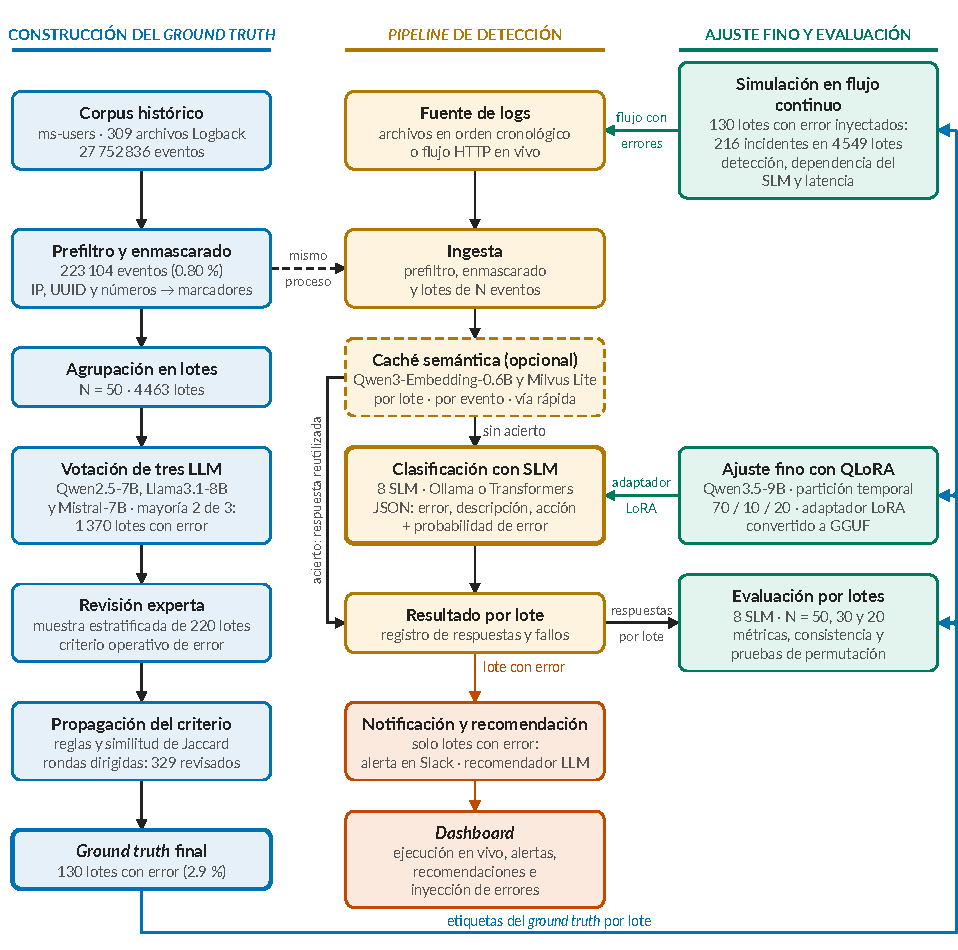
\includegraphics[width=\textwidth]{figs/metodologia/arquitectura_pipeline.pdf}
\caption{Diseño general del sistema: construcción del \textit{ground truth} (izquierda), \textit{pipeline} de detección (centro), y ajuste fino y evaluación (derecha). El borde discontinuo indica un componente opcional.}
\label{fig:arquitectura}
\end{figure}

El sistema tuvo dos usos. En la evaluación por lotes, el \textit{pipeline} recorrió el corpus histórico completo y cada respuesta fue comparada con el \textit{ground truth}, lo que permitió evaluar los modelos, los tamaños de lote y el ajuste fino. En la simulación en flujo continuo, un servidor local emitió los logs como si fueran el tráfico real del servicio, con errores inyectados en momentos conocidos, y el \textit{pipeline} los analizó en tiempo real, lo que permitió medir la detección, la latencia y la dependencia del modelo.

\subsection{Entorno de desarrollo}\label{subsec:met_entorno}

El desarrollo y la experimentación se repartieron entre dos equipos con tarjetas gráficas de fabricantes distintos, y por eso el \textit{pipeline} admite tanto la plataforma ROCm de AMD como CUDA de NVIDIA. Únicamente el ajuste fino corrió en un servidor facilitado por la DTIC, debido al alto costo computacional de reentrenar un modelo en equipos personales. La tabla~\ref{tab:met_equipos} describe los tres equipos.

\begin{table}[H]
\centering
\caption{Equipos utilizados en el desarrollo y la experimentación.}
\label{tab:met_equipos}
\footnotesize\linespread{1}\selectfont
\setlength{\tabcolsep}{4pt}
\begin{tabularx}{\textwidth}{@{}>{\raggedright\arraybackslash}p{2.1cm}>{\raggedright\arraybackslash}X>{\raggedright\arraybackslash}p{1.6cm}>{\raggedright\arraybackslash}X>{\raggedright\arraybackslash}p{1.4cm}>{\raggedright\arraybackslash}X>{\raggedright\arraybackslash}p{1.9cm}@{}}
\toprule
\textbf{Equipo} & \textbf{Rol en el estudio} & \textbf{Sistema operativo} & \textbf{CPU} & \textbf{RAM} & \textbf{GPU (VRAM)} & \textbf{Aceleración} \\
\midrule
Equipo 1 (personal) & Mayoría de las clasificaciones y la simulación & Debian & AMD Ryzen 7 3700X, 16 hilos, hasta 4.43~GHz & 24~GB & AMD Radeon RX 7900 XT (20~GB) & ROCm 7.2, PyTorch 2.13 \\
\addlinespace
Equipo 2 (personal) & Qwen3.5-9B y Ministral-3-3B con $N=30$; SmolLM2-1.7B con $N=50$ & Ubuntu & Intel Core i7-13620H, 16 hilos, hasta 4.90~GHz & 16~GB & NVIDIA GeForce RTX 4060 (8~GB) & CUDA \\
\addlinespace
Servidor de la DTIC (Google Compute Engine) & Ajuste fino del modelo & Ubuntu 22.04.5 LTS & Intel Xeon, 32 núcleos virtuales a 2.20~GHz & 125.8~GiB & NVIDIA L4 (22.5~GiB) & CUDA 13.0, \textit{driver} 580.178.04 \\
\bottomrule
\end{tabularx}
\normalsize
\end{table}

El \textit{pipeline} está escrito en Python 3.13, con Pydantic para las estructuras de logs, lotes y resultados. Ollama, ejecutado en un contenedor Docker, y Hugging Face Transformers sobre PyTorch sirvieron los modelos. Sentence-Transformers generó los \textit{embeddings}, y Milvus Lite los almacenó. Las métricas provienen de scikit-learn, las pruebas estadísticas de NumPy y SciPy, y las gráficas de Matplotlib. El ajuste fino usó las bibliotecas PEFT y bitsandbytes, y llama.cpp para convertir el adaptador al formato de Ollama. Git sirvió para el control de versiones del código.

\section{Construcción del \textit{ground truth}}\label{sec:met_gt}

No existían etiquetas que indicaran qué lotes del corpus contenían errores, así que la referencia fue construida por etapas que combinaron el pseudoetiquetado con modelos de lenguaje y la revisión de expertos. El \textit{ground truth} asigna una etiqueta a cada lote, porque un SLM evalúa un lote completo y su respuesta necesita una etiqueta del mismo nivel para compararla. La parte izquierda de la figura~\ref{fig:arquitectura} resume sus etapas, que parten del corpus de logs del servicio y de su reducción a lotes de eventos con valor diagnóstico.

\subsection{Conjunto de datos}\label{sec:met_dataset}

Los datos del trabajo provienen de \texttt{ms-users}, un microservicio Spring Boot de la DTIC que gestiona las cuentas de usuario de la universidad frente a Active Directory, LDAP, Oracle, AS400 y Google Workspace. El corpus consta de 309 archivos en formato Logback, con unos 16~GB y 27\,752\,836 eventos, que cubren del 23 de septiembre al 7 de octubre de 2026. Cada día tiene entre 21 y 22 archivos numerados desde \texttt{logFile.AAAA-MM-DD.0.log}, salvo el 7 de octubre, que llega hasta el archivo \texttt{.7}, y el conjunto incluye además el archivo activo \texttt{logFile.log}, que termina a las 09:37 de ese día. El director de la DTIC proporcionó estos registros el 13 de octubre de 2026, y a partir de esa fecha la construcción del conjunto de datos y de su \textit{ground truth} se extendió hasta el 4 de noviembre.

Casi todo el volumen del corpus es ruido de infraestructura: entre el 99.8\,\% y el 99.9\,\% corresponde a salida repetitiva que no describe operaciones del negocio. Las fuentes principales de ese ruido son los sondeos de salud de Kubernetes a \texttt{/actuator}, que Spring Security rechaza e imprime con trazas de pila de unas 115 líneas, las trazas internas de los filtros de Spring Security en nivel \texttt{TRACE} y las líneas de peticiones del \textit{framework}. Los eventos con valor de negocio son una fracción mínima y registran situaciones como rechazos por política de contraseñas, usuarios no encontrados en alguno de los sistemas externos, avisos de LDAP o cambios de contraseña exitosos.

\subsection{Prefiltrado, enmascarado y agrupación en lotes}\label{subsec:met_prefiltro}\label{subsec:met_batches}

Para reducir el volumen, el \textit{pipeline} aplica un prefiltro basado en reglas que analiza cada evento Logback y decide si conservarlo según su \textit{logger}, su nivel de severidad y su mensaje, y nunca según la dirección IP. El prefiltro mantiene los eventos de los \textit{loggers} de negocio, los de nivel \texttt{WARN}, \texttt{ERROR} o \texttt{FATAL} y las peticiones del \textit{framework}. Cada evento conservado forma una entrada cuyo texto es la línea original más su traza de pila, limitada a 15 líneas. En la práctica, el prefiltro conservó entre el 0.18\,\% y el 3.75\,\% de cada archivo, 223\,104 eventos en total, de los cuales solo unos 7\,400 son distintos.

Antes de que cualquier modelo vea el texto, el enmascarado sustituye las direcciones IP, los identificadores UUID y los números por marcadores. Esto cumple dos funciones: evita que los identificadores salgan del texto que procesan los modelos y hace que los eventos repetidos, que solo difieren en esos valores, queden idénticos.

La unidad de análisis es el lote de $N$ eventos consecutivos ya filtrados. El tamaño de lote quedó fijado en $N = 50$ con un propósito principal: establecer una línea base uniforme que permitiera comparar todos los modelos candidatos en las mismas condiciones y construir sobre ella el conjunto de referencia. Una comparación equitativa exige que todos los modelos reciban exactamente los mismos lotes, y el \textit{ground truth} fue elaborado y revisado por lotes de 50 eventos, como describen las subsecciones siguientes; cualquier otro tamaño no coincidiría con los límites de los lotes etiquetados y exigiría rehacer la votación y la revisión experta. Con $N = 50$, el corpus queda dividido en 4\,463 lotes, 4\,462 de 50 eventos y uno final de 4.

Como todos los modelos deben recibir el mismo $N$, el tamaño máximo lo fija el modelo con la ventana de contexto más pequeña: SmolLM2-1.7B-Instruct, con 8\,192 \textit{tokens}. El resto de los modelos dispone de ventanas mucho mayores, así que esta restricción solo afecta a SmolLM2-1.7B-Instruct. Para comprobar ese límite, una prueba con $N = 70$ sobre los mismos 7\,000 primeros eventos del corpus, que forman 140 lotes con $N = 50$ y 100 con $N = 70$, evaluó tres modelos de la matriz en el equipo con 8~GB de memoria de GPU. La prueba midió únicamente si los modelos podían responder en el formato esperado, y no la calidad de su detección. La tabla~\ref{tab:met_n70} muestra los resultados; los \textit{tokens} incluyen la entrada y la salida de cada llamada.

\begin{table}[H]
\centering
\caption{Prueba de viabilidad con $N = 50$ y $N = 70$ sobre los primeros 7\,000 eventos.}
\label{tab:met_n70}
\small
\begin{tabular}{@{}p{3.3cm}cp{1.8cm}p{2.6cm}p{1.6cm}p{1.6cm}@{}}
\toprule
\textbf{Modelo} & $N$ & \textbf{Respuestas válidas} & \textbf{\textit{Tokens} por lote (mediana / máx.)} & \textbf{\textit{Tokens} por evento} & \textbf{s por lote (mediana)} \\
\midrule
SmolLM2-1.7B-Instruct & 50 & 130 / 140 & 5\,380 / 5\,888 & 108.0 & 2.0 \\
 & 70 & 1 / 100 & 7\,625 / 8\,269 & 109.1 & 8.5 \\
Ministral-3-3B (BF16) & 50 & 140 / 140 & 4\,488 / 4\,757 & 89.7 & 13.8 \\
 & 70 & 100 / 100 & 6\,172 / 6\,692 & 87.9 & 16.0 \\
Qwen3.5-9B (Q6\_K) & 50 & 140 / 140 & 4\,327 / 4\,609 & 86.7 & 5.2 \\
 & 70 & 100 / 100 & 6\,005 / 6\,502 & 85.9 & 6.7 \\
\bottomrule
\end{tabular}
\normalsize
\end{table}

Con $N = 70$, el lote mediano de SmolLM2-1.7B-Instruct ocupó 7\,625 \textit{tokens}, el 93\,\% de su ventana de contexto, y solo una de sus 100 respuestas tuvo el formato JSON esperado, mientras que con $N = 50$ respondió de forma válida en 130 de los 140 lotes. Ministral-3-3B y Qwen3.5-9B respondieron sin fallos con ambos tamaños. La prueba confirma, por tanto, que $N = 70$ supera la capacidad de SmolLM2-1.7B-Instruct y no es viable para toda la matriz de modelos, sin indicar que $N = 50$ sea el mejor tamaño para cada modelo; su alcance es limitado, porque usa 7\,000 eventos y un solo equipo. Como observación secundaria, un lote más grande también tarda más en completarse: al ritmo real del servicio, de unos 0.2 eventos por segundo, un lote de 50 eventos tarda unos 250 segundos en llenarse. Los tamaños $N = 30$ y $N = 20$ sirvieron después para medir el efecto del tamaño de lote sobre los modelos, como explica la sección~\ref{sec:met_evaluacion}.

\subsection{Votación y consenso de los LLM}\label{subsec:met_votacion}\label{subsec:met_kappa}

En la primera etapa, tres LLM locales de 7\,000 a 8\,000 millones de parámetros y de familias distintas, Qwen2.5-7B, Llama3.1-8B y Mistral-7B, servidos con Ollama, votaron por separado sobre cada uno de los 4\,463 lotes de 50 eventos. Cada modelo recibió el lote como una lista numerada y devolvió un veredicto único en JSON con tres campos: si el lote contiene un error, los índices de las líneas que lo justifican y una frase de razonamiento. Un lote contaba como error si contenía al menos un evento erróneo, y un lote sin respuesta válida quedaba sin etiqueta, en lugar de asumirlo normal, para no sesgar el voto. Los modelos usaron cuantización Q4\_K\_M, temperatura 0, una ventana de contexto de 12\,288 \textit{tokens}, un máximo de 300 \textit{tokens} de respuesta y tres reintentos; ningún lote quedó truncado. El Anexo~\ref{ap:prompt_votacion} incluye el \textit{prompt} completo, y la tabla~\ref{tab:met_votos} resume la votación.

\begin{table}[H]
\centering
\caption{Votación de los tres LLM sobre los 4\,463 lotes de 50 eventos.}
\label{tab:met_votos}
\small
\begin{tabular}{@{}lrrr@{}}
\toprule
\textbf{Modelo} & \textbf{Lotes con voto de error} & \textbf{Tiempo total (h)} & \textbf{\textit{Tokens} de entrada (mediana / máx.)} \\
\midrule
qwen2.5:7b & 1\,304 & 3.7 & 4\,595 / 5\,767 \\
llama3.1:8b & 1\,396 & 2.3 & 3\,716 / 4\,836 \\
mistral:7b & 1\,400 & 4.5 & 5\,544 / 6\,942 \\
\bottomrule
\end{tabular}
\normalsize
\end{table}

Durante la votación, Mistral dejó 23 lotes sin voto porque cortaba el JSON sin cerrar la comilla ni la llave final. Como la temperatura de generación era 0 para que las respuestas fueran consistentes, los reintentos repetían el mismo corte. Para resolverlo, el analizador de respuestas incorporó un rescate mediante expresiones regulares, con el que el sistema reprocesó los 23 lotes.

El consenso corresponde a la mayoría estricta sobre los votos válidos: al menos dos de los tres modelos. Con esa regla, 1\,370 lotes (30.7\,\%) resultaron error y 3\,093 normales. El acuerdo entre los modelos fue alto: el $\kappa$ de Fleiss \cite{fleiss1971_kappa} fue 0.886, casi perfecto según la escala de Landis y Koch \cite{landis1977_kappa}, con 1\,203 lotes de error unánime, 2\,936 de normal unánime y 324 con desacuerdo. Este consenso fue solo una etiqueta preliminar, que sirvió para guiar la revisión experta.

\subsection{Revisión experta y criterio operativo}\label{subsec:met_expertos}\label{sec:met_criterio}

El consenso de los LLM podía equivocarse, así que el trabajo lo contrastó con el juicio de dos desarrolladores de la DTIC. Como revisar los 4\,463 lotes no era viable, los desarrolladores revisaron una muestra de 220, alrededor del 5\,\% del total, elegida de forma que incluyera lotes de los tres resultados posibles de la votación. Para ello, los lotes quedaron separados primero en tres grupos, llamados estratos, según cuántos modelos los habían marcado como error: error unánime, si los tres votaron error (1\,203 lotes); desacuerdo, si lo hicieron uno o dos (324), y normal unánime, si no lo hizo ninguno (2\,936). Después, un sorteo con un generador de números aleatorios de semilla fija (42) eligió 88 lotes del primer estrato, 88 del segundo y 44 del tercero; la semilla permite volver a obtener la misma muestra. El reparto no es proporcional al tamaño de los estratos: si lo fuera, la muestra tendría solo unos 16 lotes de desacuerdo, el estrato en el que los modelos no coinciden, y 145 de los 220 serían lotes que ningún modelo marcó. La figura~\ref{fig:met_muestra} muestra cómo quedó formada la muestra.

\begin{figure}[H]
\centering
% Muestreo estratificado de 220 lotes para la revisión experta (sección 3.3.4).
% Las alturas son proporcionales al número de lotes de cada estrato (8 cm = total).
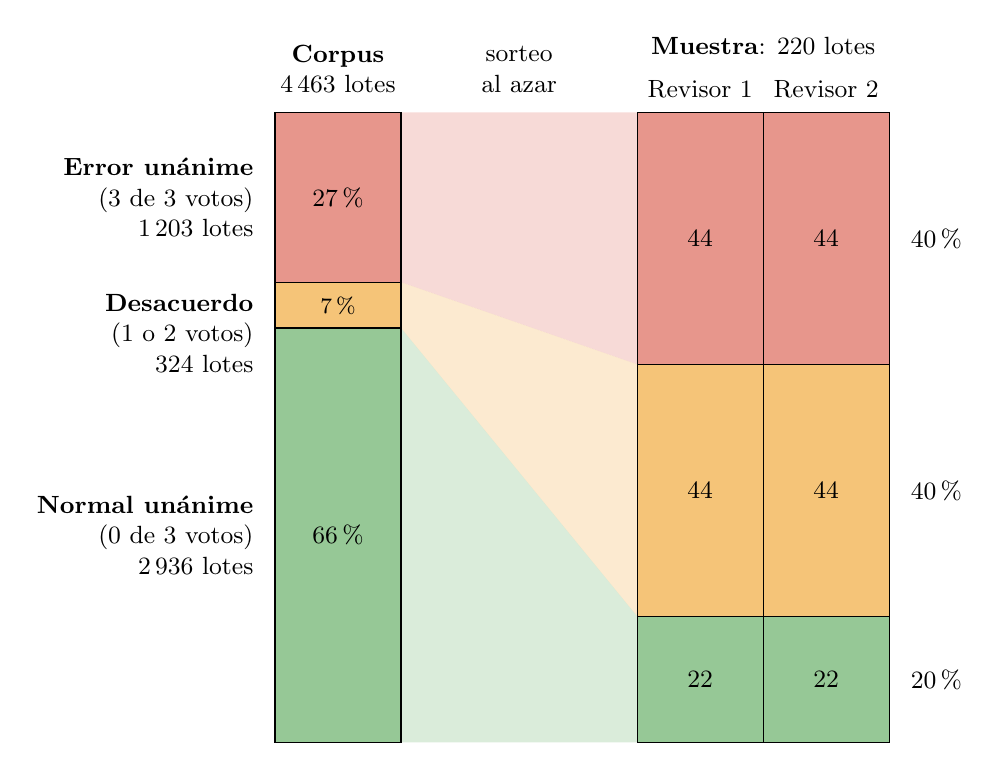
\begin{tikzpicture}[font=\small\linespread{1}\selectfont]
  \definecolor{eu}{RGB}{231,150,140}
  \definecolor{de}{RGB}{245,196,120}
  \definecolor{nu}{RGB}{150,200,150}

  % --- Conectores (sorteo), dibujados primero para quedar detrás de las barras
  \fill[eu, opacity=0.35] (1.6,8) -- (4.6,8) -- (4.6,4.8) -- (1.6,5.844) -- cycle;
  \fill[de, opacity=0.35] (1.6,5.844) -- (4.6,4.8) -- (4.6,1.6) -- (1.6,5.263) -- cycle;
  \fill[nu, opacity=0.35] (1.6,5.263) -- (4.6,1.6) -- (4.6,0) -- (1.6,0) -- cycle;

  % --- Corpus: 4 463 lotes
  \filldraw[fill=eu, draw=black] (0,5.844) rectangle (1.6,8);
  \filldraw[fill=de, draw=black] (0,5.263) rectangle (1.6,5.844);
  \filldraw[fill=nu, draw=black] (0,0)     rectangle (1.6,5.263);
  \node at (0.8,6.92) {27\,\%};
  \node at (0.8,5.55) {\footnotesize 7\,\%};
  \node at (0.8,2.63) {66\,\%};

  \node[anchor=east, align=right] at (-0.15,6.92) {\textbf{Error unánime}\\(3 de 3 votos)\\1\,203 lotes};
  \node[anchor=east, align=right] at (-0.15,5.20) {\textbf{Desacuerdo}\\(1 o 2 votos)\\324 lotes};
  \node[anchor=east, align=right] at (-0.15,2.63) {\textbf{Normal unánime}\\(0 de 3 votos)\\2\,936 lotes};

  % --- Muestra: 220 lotes, dividida en dos mitades sin solapamiento
  \foreach \x in {4.6,6.2} {
    \filldraw[fill=eu, draw=black] (\x,4.8) rectangle ++(1.6,3.2);
    \filldraw[fill=de, draw=black] (\x,1.6) rectangle ++(1.6,3.2);
    \filldraw[fill=nu, draw=black] (\x,0)   rectangle ++(1.6,1.6);
    \node at (\x+0.8,6.4) {44};
    \node at (\x+0.8,3.2) {44};
    \node at (\x+0.8,0.8) {22};
  }
  \node[anchor=west] at (7.95,6.4) {40\,\%};
  \node[anchor=west] at (7.95,3.2) {40\,\%};
  \node[anchor=west] at (7.95,0.8) {20\,\%};

  % --- Encabezados
  \node[align=center] at (0.8,8.55) {\textbf{Corpus}\\4\,463 lotes};
  \node[align=center] at (3.1,8.55) {sorteo\\al azar};
  \node at (6.2,8.85) {\textbf{Muestra}: 220 lotes};
  \node at (5.4,8.3) {Revisor 1};
  \node at (7.0,8.3) {Revisor 2};
\end{tikzpicture}

\caption{Muestra estratificada de 220 lotes para la revisión experta. La altura de cada bloque es proporcional a su número de lotes.}
\label{fig:met_muestra}
\end{figure}

Cada revisor recibió la mitad de la muestra, 110 lotes con 44 de error unánime, 44 de desacuerdo y 22 de normal unánime, sin lotes en común con el otro. Los lotes llegaron en un archivo CSV con una fila por lote, que contenía el texto completo de sus 50 eventos, las líneas que los modelos habían señalado como error, sus votos y el razonamiento de cada uno. El revisor leía el lote, decidía si contenía una falla del servicio y anotaba 1 (error) o 0 (normal), con una nota opcional que justificara su decisión. Por ejemplo, en un lote que dos de los tres modelos marcaron como error, el revisor anotó 0 con la nota ``son logs de información cuando un enlace está vencido o validaciones de usuario''.

Entre los dos contradijeron al consenso en 33 de los 88 lotes de error unánime (37.5\,\%), en 24 de los 88 de desacuerdo (27.3\,\%) y en ninguno de los 44 de normal unánime, con el mismo patrón en ambas mitades (16 y 17 de sus 44 lotes de error unánime): los modelos marcaban como error condiciones que la institución considera normales, como el rechazo de una contraseña por la política de seguridad o la búsqueda de un usuario que no existe. Por ello, los revisores proporcionaron el criterio operativo de la tabla~\ref{tab:met_criterio}, que distingue las fallas del sistema de las condiciones funcionales que el servicio maneja correctamente.

\begin{table}[H]
\centering
\caption{Criterio operativo de error acordado por los revisores.}
\label{tab:met_criterio}
\small
\begin{tabular}{@{}p{7.2cm}p{7.2cm}@{}}
\toprule
\textbf{Es error (falla del sistema)} & \textbf{Es normal (condición funcional manejada)} \\
\midrule
Respuestas HTTP 5xx & Respuestas HTTP 4xx del cliente \\
Excepciones no controladas de la aplicación & Usuario no encontrado en AD, Google, LDAP u Oracle, y siempre en AS400 (decisión explícita) \\
Fallos al crear o actualizar cuentas por causa interna & Rechazo por política de contraseñas \\
Fallas de la API de AD o de conectividad & Entidades que ``ya existen'' \\
Errores de base de datos o del \textit{pool} de conexiones, fallo al iniciar el servicio y correo no enviado & Operaciones exitosas \\
\bottomrule
\end{tabular}
\normalsize
\end{table}

Con este criterio, solo el 12.5\,\% de los lotes de error unánime (11 de 88) resultaron error según los desarrolladores: los revisores contradijeron ahora al consenso en 77 de esos 88 lotes, frente al 6.8\,\% de error en los de desacuerdo y al 0\,\% en los de normal unánime. Como esta es la única muestra aleatoria del proceso, es la que permite estimar la tasa de error de cada estrato en el corpus completo.

\subsection{Propagación del criterio y \textit{ground truth} final}\label{subsec:met_propagacion}

Revisar los 4\,463 lotes no era viable, así que el criterio experto fue extendido al resto de forma reproducible, con registro del origen de cada etiqueta. Cada lote pasó, en orden, por las siguientes reglas, y decidió la primera que se cumplía. Si un experto lo había revisado, valía su etiqueta. Si ningún LLM había votado error, el lote quedaba como normal, una regla que la muestra respalda, porque ninguno de los 44 lotes de normal unánime fue contradicho. Si algún evento cumplía una regla de error derivada del criterio de la tabla~\ref{tab:met_criterio} (respuestas 5xx, el mensaje ``Failed to complete request'', errores al crear o actualizar cuentas o errores de la API de AD, con exclusiones para ``ya existe'' y la política de contraseñas), el lote quedaba como error. Si todo lo señalado por los modelos era ``usuario no encontrado'' de AS400, el lote era normal. Por último, si el lote se parecía a lotes ya revisados, heredaba su etiqueta cuando había una mayoría clara.

Para esta última regla, cada lote quedó descrito con una firma: el conjunto de tipos de evento (nivel, \textit{logger} y mensaje normalizado) de las líneas que habían señalado los LLM. La similitud entre dos lotes es el coeficiente de Jaccard entre sus firmas, cuya definición formal se presentó en el capítulo~\ref{cap:antecedentes} \cite{manning2008_ir}, y solo contaron los lotes revisados con una similitud de al menos 0.5. Cada uno de ellos aportó un voto por su etiqueta, ponderado por su similitud, y la pureza es la fracción de ese voto ponderado que obtiene la etiqueta mayoritaria. El lote heredaba la etiqueta solo si la pureza era de al menos 0.8; si los lotes parecidos estaban divididos, no había mayoría clara y el lote no recibía etiqueta por esta vía. El umbral de 0.5 resultó de comparar los valores 1.0, 0.7, 0.5 y 0.35 mediante una validación \textit{leave-one-out} sobre los primeros 176 lotes revisados, como compromiso entre la cantidad de lotes cubiertos y el acierto; como esa elección usó los mismos datos con que se mide, la validación es optimista.

Si ninguna regla aplicaba, el lote no recibía el voto de los LLM, sino que pasaba a revisión. Así hubo tres rondas dirigidas, con 91, 17 y 1 representantes de grupos de lotes idénticos que cubrieron 110, 22 y 1 lotes. En total, los expertos revisaron 329 lotes (7.4\,\%), de los cuales 39 resultaron error y 290 normales.

El resultado es una etiqueta para cada uno de los 4\,463 lotes; la tabla~\ref{tab:met_origen} muestra el origen de las etiquetas. Los 130 lotes con error (2.9\,\%) provienen solo de la revisión directa (39) y de las reglas de error (91); la similitud con lotes revisados únicamente asignó etiquetas normales. Frente al consenso de los LLM, los expertos eliminaron 1\,241 de sus 1\,370 positivos y añadieron un error nuevo, y ambas referencias coinciden solo en el 72.2\,\% de los lotes. Esta etiqueta, denominada \texttt{final\_is\_error}, es la referencia de todas las evaluaciones del trabajo.

\begin{table}[H]
\centering
\caption{Origen de las etiquetas del \textit{ground truth} final por lote ($N=50$).}
\label{tab:met_origen}
\small
\begin{tabular}{@{}lr@{}}
\toprule
\textbf{Origen} & \textbf{Lotes} \\
\midrule
Ningún LLM votó error & 2\,892 \\
Similitud con un lote revisado & 1\,093 \\
Revisión experta & 329 \\
Regla de error & 91 \\
Regla de AS400 (normal) & 58 \\
\midrule
\textbf{Total} & \textbf{4\,463} \\
\bottomrule
\end{tabular}
\normalsize
\end{table}

La diferencia entre el voto de los LLM y el criterio experto muestra la dificultad central del problema: un modelo genérico interpreta cualquier excepción o línea de nivel \texttt{ERROR} como una falla, mientras que la institución considera muchas de ellas resultados normales del negocio.

\section{Ingesta y clasificación con SLM}\label{sec:met_arquitectura}

El \textit{pipeline} consta de cuatro módulos: un lector que entrega los eventos, un modelo que analiza cada lote, un escritor que registra cada resultado y un servicio de notificaciones. Esta organización permitió usar el mismo flujo tanto sobre los archivos históricos como sobre un flujo HTTP en vivo, y cambiar el modelo o el tipo de caché sin modificar el resto.

El lector obtiene los eventos de los archivos de log, en orden cronológico para su reproducibilidad, o de un flujo HTTP que simula la operación en vivo. A cada evento le aplica el mismo prefiltro y enmascarado con que fue construido el \textit{ground truth}, descritos en la sección~\ref{subsec:met_prefiltro}, y los agrupa en lotes de $N$ eventos filtrados.

\subsection{Clasificación}\label{subsec:met_clasificacion}

El \textit{pipeline} envía cada lote al SLM como una lista numerada de eventos, acompañada de un mensaje de sistema fijo que define la tarea, el formato de respuesta y las condiciones que no cuentan como error, como las solicitudes erróneas, las excepciones de validación de contraseñas o los usuarios no encontrados. El modelo responde un objeto JSON corto con tres campos: si hay error, una descripción breve y una acción recomendada. El Anexo~\ref{ap:prompt_slm} incluye el mensaje de sistema completo. El \textit{pipeline} admite dos motores de inferencia intercambiables: Ollama, para los modelos cuantizados en formato GGUF, y Hugging Face Transformers, para los modelos en su formato original. Ambos usan temperatura 0 y decodificación voraz para obtener clasificaciones consistentes, con el razonamiento extendido de los modelos desactivado y un máximo de 512 \textit{tokens} de respuesta.

\tema{Probabilidad de error}

Además de la respuesta binaria, el \textit{pipeline} registra la probabilidad de error de cada lote, obtenida de las probabilidades que el modelo asigna a los \textit{tokens} \texttt{true} y \texttt{false} en la posición donde escribe su decisión. En Transformers, el cálculo parte de los \textit{logits}, y en Ollama, de las probabilidades logarítmicas de las alternativas más probables que devuelve el servidor. Esta puntuación permite construir las curvas ROC y de precisión-\textit{recall} y elegir umbrales de decisión distintos de 0.5.

\tema{Robustez}

Los modelos pequeños no siempre respetan el formato pedido, así que el \textit{pipeline} incorpora tres protecciones. La primera es un analizador que repara las respuestas mal formadas, como saltos de línea sin escapar, comillas sin cerrar, claves sin comillas o un JSON cortado, y que en algunos modelos recuperó el 100\,\% de las respuestas que de otro modo se habrían perdido. La segunda es un registro de fallos que guarda la entrada y la respuesta cruda de cada lote que no puede procesarse, sin detener la ejecución. La tercera es un límite de \textit{tokens} de salida y un tiempo máximo por petición, que detienen las generaciones descontroladas; en una ocasión, un modelo llegó a generar 141\,000 \textit{tokens} para un solo lote.

\subsection{Modelos evaluados}\label{sec:met_slm}

Para el clasificador, el trabajo seleccionó ocho SLM, de 1\,000 a 9\,000 millones de parámetros y de familias y desarrolladores distintos. El criterio de selección fue que fueran SLM capaces de ejecutarse de forma local con requerimientos acotados de memoria de video (VRAM), para que pudieran funcionar en equipos con una sola tarjeta gráfica. La tabla~\ref{tab:met_modelos} lista los modelos, el motor con que corrió cada uno, su formato y la memoria de video que requirieron.

\begin{table}[H]
\centering
\caption{Modelos evaluados como clasificadores y memoria de video requerida.}
\label{tab:met_modelos}
\small
\begin{tabular}{@{}lllr@{}}
\toprule
\textbf{Modelo} & \textbf{Motor} & \textbf{Formato} & \textbf{VRAM (GiB)} \\
\midrule
Phi-3.5-mini (3.8B) & Transformers & Pesos originales & 10.6 \\
Gemma-3-4B & Transformers & Pesos originales & 9.6 \\
Ministral-3-3B & Ollama & BF16 & 9.3 \\
Qwen3.5-9B & Ollama & Q6\_K & 8.4 \\
Granite-4.1-3B & Transformers & Pesos originales & 6.9 \\
Ling-3.0-tiny & Ollama & Q4\_K\_M & 5.0 \\
SmolLM2-1.7B-Instruct & Transformers & Pesos originales & 4.9 \\
Llama-3.2-1B \textit{log-analyzer} & Ollama & Q4\_K\_M & 1.7 \\
\bottomrule
\end{tabular}
\normalsize
\end{table}

Todos los modelos recibieron el mismo \textit{prompt}, el mismo enmascarado, el mismo límite de \textit{tokens} de salida y decodificación voraz, en la que el modelo toma siempre el siguiente \textit{token} con mayor probabilidad; así, las diferencias entre ellos se deben solo al modelo. Un modelo requirió un tratamiento especial: el Llama-3.2-1B \textit{log-analyzer}, un ajuste público orientado a logs, solo funcionó a través de Ollama con su propia plantilla de conversación, porque con Transformers repetía los logs en lugar de responder.

\section{Caché semántica}\label{sec:met_cache}

Los logs del servicio se repiten mucho: entre los 223\,104 eventos conservados hay solo unos 7\,400 distintos. Esto sugiere que muchas consultas al modelo podrían evitarse reutilizando respuestas ya obtenidas, y para comprobarlo el \textit{pipeline} incorpora una caché opcional con tres variantes, comparadas en la simulación que describe la sección~\ref{sec:met_simulacion}.

\tema{Modelo de \textit{embeddings}}

El modelo Qwen3-Embedding-0.6B convierte los textos en vectores \cite{zhang2025_qwen3emb}. Los vectores quedan truncados a 512 dimensiones, aprovechando que el modelo admite representaciones \textit{Matryoshka} \cite{kusupati2022_matryoshka}, vuelven a normalizarse y no llevan instrucción. El modelo tiene un límite de 8\,192 \textit{tokens}, suficiente para que tanto un evento, de unos 85 \textit{tokens}, como un lote completo de 50 eventos quepan enteros sin truncarse. Cada vector de 512 dimensiones ocupa 2~KB y queda almacenado en Milvus Lite.

\tema{Caché por lote}

En esta variante, cada lote completo se convierte en un \textit{embedding}, y la caché busca el lote guardado más parecido según la similitud del coseno, que compara la dirección de los vectores con independencia de su magnitud. Si esa similitud supera un umbral, la caché reutiliza su respuesta sin llamar al SLM; si no, el SLM responde y la caché guarda el lote.

\tema{Caché por evento}

En esta variante, la decisión ocurre evento a evento, con dos estados. Un evento pasa a ser \emph{normal conocido} cuando aparece en un lote que el SLM respondió como normal. Si el SLM marca un lote como error, sus eventos todavía desconocidos quedan como \emph{sospechosos}, porque el modelo no indica qué línea contiene el error y la caché asume que está entre los eventos nuevos. Un lote evita al SLM solo si todos sus eventos son normales conocidos; cualquier evento desconocido o sospechoso lo envía al modelo, y un evento sospechoso que luego aparece en un lote normal pasa a normal. En la variante exacta, la caché compara cada evento por su texto enmascarado sin la marca de tiempo y guarda las claves en memoria; en la variante por similitud, un evento nunca visto toma el estado del evento guardado más parecido si la similitud del coseno supera el umbral. La figura~\ref{fig:met_cache_evento} ilustra esta lógica.

\begin{figure}[H]
\centering
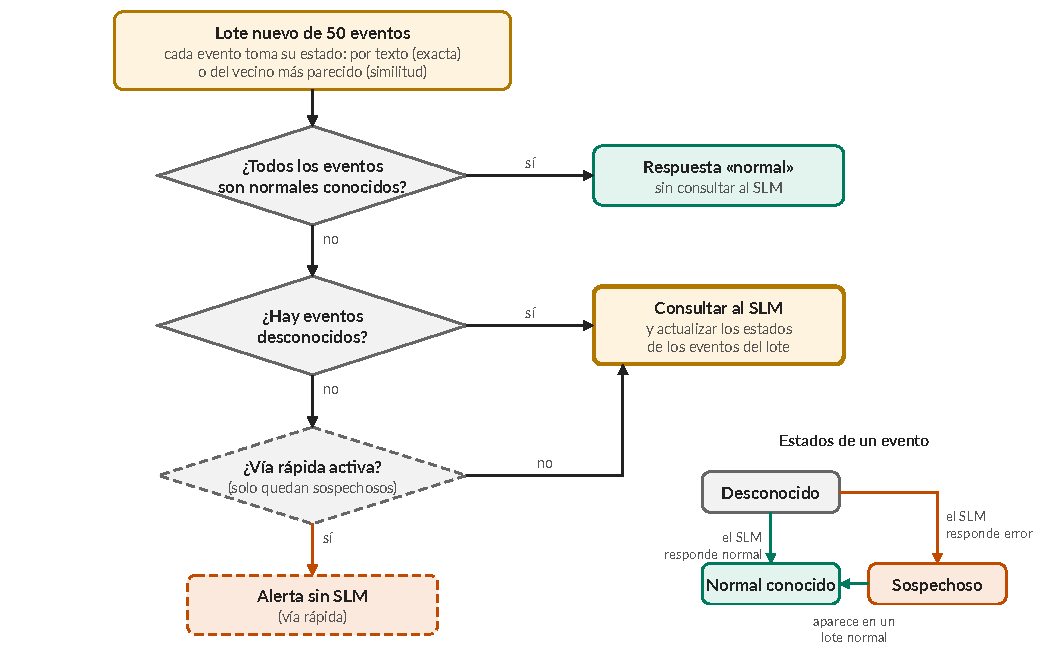
\includegraphics[width=\textwidth]{figs/metodologia/cache_evento.pdf}
\caption{Lógica de decisión de la caché por evento.}
\label{fig:met_cache_evento}
\end{figure}

\tema{Vía rápida}

La vía rápida extiende la caché por evento: si un lote no tiene eventos desconocidos y contiene al menos uno sospechoso, la alerta sale directamente, sin llamar al SLM. La simulación probó su variante exacta y los umbrales de similitud de 0.99 y 0.995.

\tema{Elección de los umbrales}

Los umbrales de similitud quedaron definidos antes de la simulación, a partir de las respuestas de Qwen3.5-9B sobre el corpus original de 4\,463 lotes y 130 errores. Para la caché por lote, los umbrales fueron 0.90, 0.95, 0.97, 0.98, 0.99 y 0.995, y para la caché por evento, 0.85, 0.90, 0.95, 0.97, 0.98, 0.99 y 0.995. El rango cubre desde casi no usar la caché hasta usarla casi siempre, y excluye los extremos sin interés: 0.999 en la caché por lote, que ya no evita llamadas, y 0.80 en la caché por evento, que pierde demasiados errores.

\section{Ajuste fino con QLoRA}\label{sec:met_finetuning}

Una evaluación preliminar de los SLM mostró que detectaban los errores reales, pero marcaban como error muchas condiciones que la institución considera normales. Para alinear el criterio del modelo seleccionado, Qwen3.5-9B, con el del \textit{ground truth} experto y reducir las falsas alarmas, el modelo recibió un ajuste fino mediante QLoRA \cite{dettmers2023_qlora}.

\subsection{Datos de entrenamiento, validación y prueba}

Los datos son los lotes de 50 eventos con su etiqueta \texttt{final\_is\_error}, presentados con el mismo \textit{prompt} y el mismo formato de respuesta JSON que usa el \textit{pipeline}. El corpus quedó dividido en el tiempo, por la posición de los lotes, con un lote de separación entre partes, para que la prueba simulara datos futuros y ningún texto de un lote de prueba apareciera en el entrenamiento. La tabla~\ref{tab:met_particion} muestra la partición.

\begin{table}[H]
\centering
\caption{Partición temporal del corpus para el ajuste fino.}
\label{tab:met_particion}
\small
\begin{tabular}{@{}llrr@{}}
\toprule
\textbf{Parte} & \textbf{Lotes del corpus} & \textbf{Ejemplos} & \textbf{Con error} \\
\midrule
Entrenamiento & 0--3\,123 (70\,\%) & 693 & 77 \\
Validación & 3\,125--3\,569 (10\,\%) & 224 & 24 \\
Prueba & 3\,571--4\,462 (20\,\%) & 892 (todos) & 29 \\
\bottomrule
\end{tabular}
\normalsize
\end{table}

Los negativos difíciles son lotes normales que el modelo sin ajustar marcaba como error, es decir, sus propias falsas alarmas, y los negativos fáciles, lotes que el modelo identificaba correctamente como normales. El conjunto de entrenamiento incluyó los 77 lotes con error, 423 negativos difíciles y 193 negativos fáciles, en una proporción de ocho negativos por cada error. La validación incluye los 24 errores de su tramo y 200 lotes normales, y la prueba conserva todos los lotes de su tramo para medir el desempeño con la prevalencia real.

\subsection{Entrenamiento y despliegue}

El ajuste aplicó QLoRA \cite{dettmers2023_qlora}: el modelo base Qwen3.5-9B quedó cargado en 4 bits con NormalFloat (NF4), a partir de una copia ya cuantizada para no agotar la RAM, y sobre él se entrenó un adaptador LoRA de rango 16, $\alpha = 32$ y \textit{dropout} de 0.05 en todas las capas lineales, con unos 43 millones de parámetros entrenables, el 0.48\,\% del modelo. Esta configuración está en línea con lo observado en una búsqueda de hiperparámetros sobre modelos de 7\,000 a 65\,000 millones de parámetros, donde un \textit{dropout} de 0.05 resultó útil en los modelos más pequeños y el rango no influyó en el desempeño final cuando el adaptador se aplicaba a todas las capas \cite{dettmers2023_qlora}. La pérdida estaba ponderada para compensar el desbalance de clases: los ejemplos con error pesan 4 veces, los negativos difíciles 2 veces y el \textit{token} de decisión (\texttt{true} o \texttt{false}), 10 veces, porque es el que determina la clasificación. El entrenamiento usó una tasa de aprendizaje de $10^{-4}$, dos épocas, acumulación de gradientes de 8 ejemplos (174 pasos) y hasta 6\,144 \textit{tokens} por ejemplo. Cada 20 pasos, el proceso validó el modelo y guardó un punto de control, y al final conservó el de menor pérdida de validación.

El entrenamiento corrió en el servidor facilitado por la DTIC, duró 10.6~horas y alcanzó un máximo de 19.1~GiB de memoria de GPU, dentro de los 22.5~GiB de su tarjeta NVIDIA L4. La pérdida de validación bajó de 0.239, tras el primer cuarto de época, a un mínimo de 0.166 en la época 1.6, y se mantuvo estable hasta el final (0.167).


Llama.cpp convirtió el adaptador al formato GGUF, con un tamaño de 86~MB, y un archivo de configuración de Ollama lo aplica sobre el mismo Qwen3.5-9B Q6\_K usado en todas las evaluaciones. Así, la comparación entre el modelo base y el ajustado cambia solo el adaptador. El modelo ajustado clasificó el corpus completo con la misma configuración que el modelo base: 4\,463 lotes en 3.5 horas, unos 2.8 segundos por lote, sin respuestas inválidas.

\section{Notificación, recomendación y \textit{dashboard}}\label{sec:met_notificacion}\label{sec:met_dashboard}

La detección se complementa con los mecanismos que llevan el resultado a las personas responsables. Un proceso en segundo plano actúa solo sobre los lotes con error válidos, para que el ciclo de clasificación nunca tenga que esperarlo. Por cada lote con error, envía una alerta corta a un canal de Slack, la plataforma de mensajería elegida por su popularidad en equipos de desarrollo y su uso recurrente en la DTIC, con el modelo, la ejecución, el lote, la probabilidad de error y los archivos de origen, y solicita a un LLM separado, el recomendador, una causa probable y una acción sugerida. El recomendador es un modelo configurable servido por Ollama; en este trabajo fue Qwen2.5-7B, con temperatura 0.2, una ventana de contexto de 8\,192 \textit{tokens}, un máximo de 600 \textit{tokens} de respuesta y un límite de 12\,000 caracteres de entrada para que el lote quepa en la ventana. Las recomendaciones solo aparecen en el \textit{dashboard} y no en la alerta, y el recomendador sugiere sin ejecutar ninguna acción. La recomendación es un apoyo al análisis de causa raíz que realiza el equipo de operación, y no un análisis de causa raíz automático: propone una causa probable a partir de los eventos del lote, sin correlacionar métricas ni trazas, para que el responsable no parta de cero. La calidad de las recomendaciones no fue evaluada formalmente.

El \textit{dashboard} es una interfaz web propia que sigue una ejecución en vivo y muestra su estado, las métricas, los lotes fallidos, las alertas y las recomendaciones. También permite inyectar errores simulados en un \textit{pipeline} en ejecución: antes de cada lote, el \textit{pipeline} agrega los errores pendientes en posiciones aleatorias, con la marca de tiempo y el hilo de un evento vecino, y registra si el lote que los contiene fue detectado. La figura~\ref{fig:met_dashboard} muestra su interfaz.

\figpendiente{fig:met_dashboard}{Interfaz del \textit{dashboard} durante una ejecución.}{Captura de pantalla del \textit{dashboard} con una ejecución en curso: estado de la ejecución, métricas, alertas, tarjeta de recomendaciones y tarjeta de inyección de errores.}

\figpendiente{fig:met_slack}{Ejemplo de alerta enviada a Slack.}{Captura de una alerta ``Error detectado'' en el canal de Slack, con modelo, ejecución, lote, probabilidad de error y archivos de origen.}

\section{Evaluación por lotes}\label{sec:met_evaluacion}

La evaluación buscó responder tres preguntas: qué modelo detecta mejor los errores, cuánto influye el tamaño del lote y si el ajuste fino mejora al modelo base. Para que las diferencias dependieran solo del modelo y del tamaño de lote, todas las ejecuciones usaron el mismo filtro, el mismo enmascarado y el mismo \textit{prompt}. Para ello, cada modelo procesó el corpus completo con tres tamaños de lote: $N = 50$ (4\,463 lotes), $N = 30$ (7\,437 lotes) y $N = 20$ (11\,156 lotes). Esto permitió medir si dar al modelo más o menos contexto por decisión mejora o empeora su desempeño.

\subsection{Métricas}\label{subsec:met_metricas}

Cada lote del modelo fue comparado con el lote correspondiente del \textit{ground truth} para calcular la precisión, el \textit{recall}, el $F_1$, la exactitud, la \textit{balanced accuracy}, la especificidad, el MCC y el AUC de la curva ROC, junto con las matrices de confusión y las curvas ROC y de precisión-\textit{recall}. La curva de precisión-\textit{recall} recorre todos los umbrales sobre la probabilidad de error, y su resumen es la AP, cuya referencia es la de un clasificador al azar, igual a la proporción de errores (0.029 con $N = 50$). Como solo el 2.9\,\% de los lotes son errores, la exactitud resulta engañosa, y los criterios principales fueron el MCC, la \textit{balanced accuracy} y la precisión \cite{chicco2020_mcc}.

\begin{figure}[H]
\centering
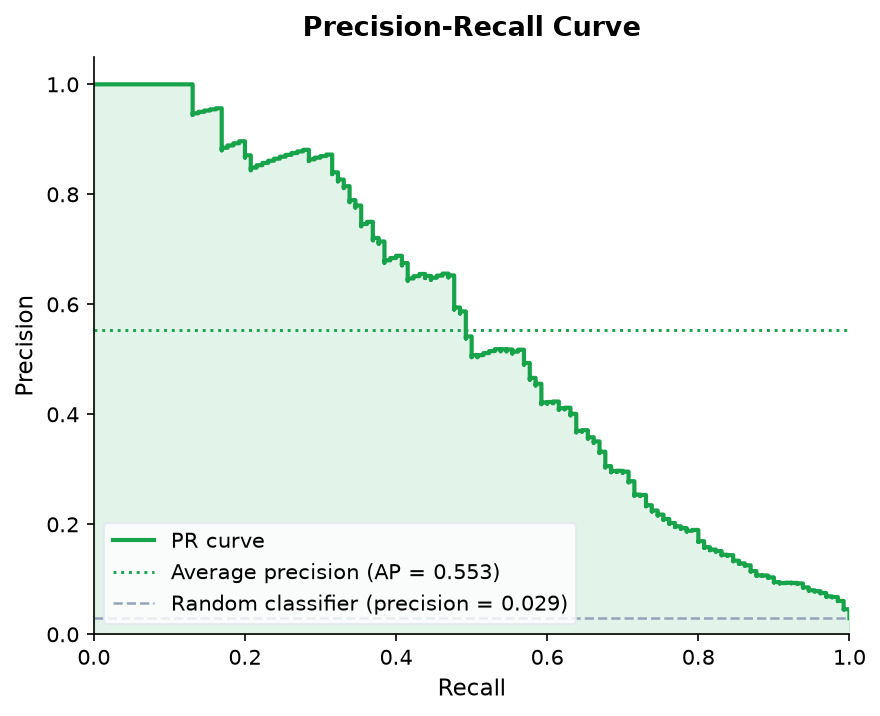
\includegraphics[width=0.75\textwidth]{figs/metodologia/curva_pr_ejemplo.jpeg}
\caption{Ejemplo de curva de precisión-\textit{recall} (Ling-3.0-tiny, $N = 50$), con su precisión promedio (AP = 0.553) y la referencia del clasificador al azar, igual a la proporción de errores (0.029).}
\label{fig:met_pr_ejemplo}
\end{figure}


\subsection{Consistencia al reducir el tamaño de lote}

Al reducir el tamaño de lote, el modelo decide con menos contexto, y nada garantiza que conserve la misma clasificación que con lotes de 50 eventos. Como un lote de 30 o de 20 eventos no coincide con ningún lote de 50, no es posible comparar directamente ambas respuestas sobre el mismo contenido. Por ello, cada lote pequeño quedó asociado al lote de 50 con el contenido más parecido: el mismo modelo de \textit{embeddings} de la caché convirtió el texto enmascarado de ambos, completo y sin truncar, y el vecino más cercano por similitud del coseno ($k = 1$) sirvió de pareja.

La referencia de cada lote pequeño fue la respuesta que el mismo modelo generó, con $N = 50$, a su vecino; así, la prueba mide si un modelo repite su propio veredicto ante un contenido equivalente, y no si acierta. La métrica principal fue el kappa de Cohen \cite{cohen1960_kappa}, que mide el acuerdo por encima del esperado por azar, acompañado del MCC y de dos proporciones: la de alertas de $N = 50$ que el modelo repite con el lote pequeño y la de alertas del lote pequeño cuya referencia también era una alerta. Si la respuesta de $N = 50$ falló, el lote quedó sin referencia y fuera de la comparación; si falló la del lote pequeño, contó como desacuerdo.

Para saber si el acuerdo de cada modelo superaba al azar, el análisis aplicó una \uline{prueba de permutación} en la que la serie de referencias se desplaza circularmente frente a las respuestas, lo que conserva la correlación entre lotes consecutivos y solo rompe su alineación \cite{good2005_permutation}, con 10\,000 permutaciones y corrección de Holm entre los ocho modelos \cite{holm1979_sequential}. Las diferencias de consistencia entre modelos pasaron por el mismo procedimiento global y por pares de la sección~\ref{subsec:met_significancia}.

\subsection{Significancia estadística}\label{subsec:met_significancia}

Para saber si las diferencias entre modelos eran reales o fruto del azar, el análisis siguió un procedimiento en dos pasos. En el primero, para cada métrica, una prueba de permutación pareada entre todos los modelos contrastó la hipótesis nula de que todos rinden igual. Bajo esa hipótesis, las predicciones de los modelos sobre un mismo lote son intercambiables, así que la distribución del estadístico puede obtenerse reordenándolas al azar \cite{good2005_permutation}. Como examinar todas las reordenaciones posibles no es viable, el análisis tomó una muestra aleatoria de 10\,000, siguiendo la aproximación de Monte Carlo \cite{good2005_permutation}: en cada una, las predicciones de los modelos cambiaron de lugar al azar dentro de cada lote, y el estadístico fue la diferencia entre el mejor y el peor valor de la métrica. En el segundo paso, solo para las métricas en que la prueba global rechazó la hipótesis, la misma prueba comparó los modelos por pares. Como el análisis probó muchas métricas y pares a la vez, el procedimiento de Holm corrigió los valores $p$ \cite{holm1979_sequential}.

Los lotes en que un modelo no dio una respuesta válida contaron como fallos de ese modelo: falso negativo si el lote tenía un error y falso positivo si era normal, con la peor probabilidad posible para el AUC. Así, cada modelo quedó evaluado sobre todos los lotes, en lugar de quitar un lote a todos cuando uno solo fallaba en él. Los intervalos de confianza del 95\,\% provienen de un \textit{bootstrap} circular por bloques de 2\,000 remuestreos. A diferencia del \textit{bootstrap} ordinario, que remuestrea observaciones sueltas, este método remuestrea con reemplazo bloques de observaciones consecutivas, lo que lo hace adecuado para secuencias en las que las observaciones vecinas están correlacionadas, como ocurre con los lotes de un mismo registro. En la variante circular, los lotes forman un círculo, y un bloque que llega al último lote continúa desde el primero, con lo que los lotes de los extremos no quedan con menos peso que el resto \cite{politis1991_circular}. Su consistencia exige que la longitud de los bloques crezca con el número de lotes, pero en una proporción cada vez menor de ese número; en este trabajo, la longitud es la raíz cúbica del número de lotes, que cumple esa condición.

\subsection{Evaluación del ajuste fino}

El modelo ajustado y el modelo base fueron comparados solo sobre los 892 lotes de prueba, con 29 errores; los lotes de entrenamiento quedaron fuera de la calificación, y los de validación solo sirvieron para elegir el umbral. Cada modelo tuvo dos variantes: su respuesta tal cual y una variante con umbral, que marca error cuando la probabilidad de error supera el umbral que maximiza el MCC en los 445 lotes de validación (0.959 para el modelo base y 0.978 para el ajustado). Con clases desbalanceadas, el umbral por defecto de 0.5 suele no ser el adecuado, y ajustarlo compensa el desbalance sin necesidad de reentrenar el modelo \cite{esposito2021_ghost}. El umbral solo cambia la decisión y no la probabilidad, así que el AUC y la AP son iguales con y sin umbral. La significancia siguió el mismo procedimiento de permutaciones y corrección de Holm.

\section{Simulación en flujo continuo con errores inyectados}\label{sec:met_simulacion}\label{sec:met_inyeccion}

La evaluación por lotes mide la capacidad del modelo para clasificar, pero no cómo se comporta el sistema completo cuando los logs llegan en tiempo real. Para comprobarlo, la simulación inyectó errores reales del \textit{ground truth} en un flujo de logs que el \textit{pipeline} analizó en tiempo real, y midió la tasa de detección, la latencia desde que el error aparece hasta que sale la alerta y las falsas alarmas. La prueba permite verificar si, a medida que crece la base de \textit{embeddings}, el sistema depende menos del SLM para detectar los errores más rápido, y cuánto mejora el flujo con el SLM ajustado. La figura~\ref{fig:met_simulacion} muestra el esquema del experimento.

\begin{figure}[H]
\centering
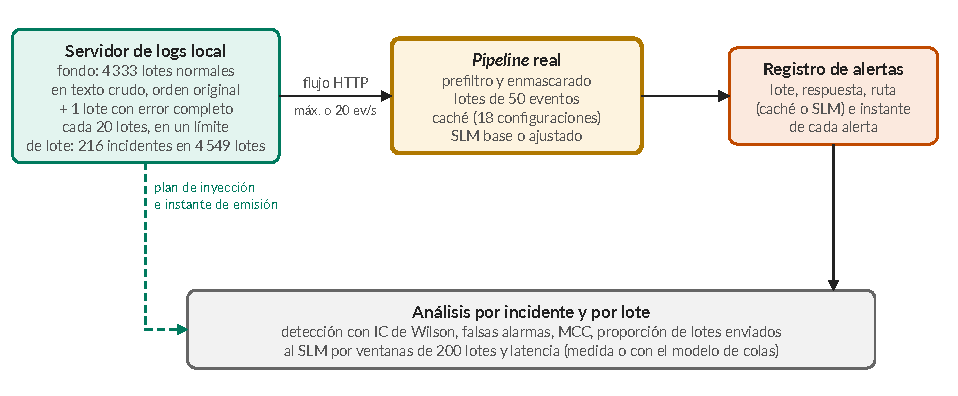
\includegraphics[width=\textwidth]{figs/metodologia/simulacion.pdf}
\caption{Esquema de la simulación en flujo continuo.}
\label{fig:met_simulacion}
\end{figure}

\subsection{Construcción del flujo}

El fondo del flujo son los eventos de los 4\,333 lotes de 50 que el \textit{ground truth} considera normales (216\,650 eventos), en su orden original y como texto crudo, tal como los escribió el servicio. Los errores a inyectar provienen de los 130 lotes con error del \textit{ground truth}: cada uno aportó un incidente formado por el lote completo, con sus 50 eventos, en total 130 incidentes con 6\,500 eventos. La inyección usó el lote entero porque la etiqueta del \textit{ground truth} corresponde al lote completo y no a cada evento. Antes de usarlos, una comprobación confirmó que el filtro del \textit{pipeline} conservaba todos sus eventos.

Un servidor de logs local emitió el fondo por HTTP e insertó un incidente cada 20 lotes, siempre en un límite de lote; así, cada incidente ocupa exactamente un lote del \textit{pipeline} y cada lote del flujo es un lote del corpus, sea un incidente o un lote normal del fondo. El primer incidente llegó después de los primeros 20 lotes, y el flujo completo sumó 216 incidentes en 4\,549 lotes. Cada lote con error constituye su propio tipo de incidente, y el servidor recorrió los tipos en orden rotativo con una semilla fija, lo que dio 130 primeras apariciones y 86 segundas, que reinyectan el mismo lote. Las líneas inyectadas conservaron su hilo original y recibieron la marca de tiempo de la línea anterior del fondo, con lo que nada las distinguía del tráfico real, y el servidor registró el instante exacto en que escribió cada incidente.

El \textit{pipeline} leyó el flujo por el mismo camino de producción, con filtro, enmascarado, lotes de 50, clasificación y alerta, y registró el instante de cada alerta en un archivo. Una verificación sobre los primeros 60\,000 eventos confirmó que la posición de cada evento en el flujo coincidía con su posición en el corpus filtrado, así que la verdad de cada lote fue exacta: un lote del flujo es error si y solo si es un incidente inyectado, lo que da 216 lotes con error y 4\,333 normales.

\subsection{Métodos comparados}

La simulación usó Qwen3.5-9B, el mejor modelo de la evaluación por lotes, en dos versiones: el modelo base y el mismo modelo con el adaptador LoRA descrito en la sección~\ref{sec:met_finetuning}. Ambos procesaron lotes de 50 eventos con el mismo \textit{prompt} y enmascarado. Con cada modelo, la simulación comparó cinco métodos: el SLM solo, que analiza todos los lotes y sirve de referencia; la caché por lote, con seis umbrales; la caché por evento exacta; la caché por evento con similitud, con siete umbrales; y la vía rápida, en sus variantes exacta, 0.99 y 0.995, con los umbrales descritos en la sección~\ref{sec:met_cache}. En total, cada modelo corrió 18 configuraciones.

Los dos modelos recibieron exactamente el mismo flujo, con el mismo plan de inyección y los mismos rangos de eventos por lote, lo que hace comparables sus métricas de detección. El modelo base corrió en el equipo 2 y el ajustado en el equipo 1 de la tabla~\ref{tab:met_equipos}, ambos equipos personales con una sola tarjeta gráfica. Además, el flujo recorre todo el corpus e incluye, por tanto, los lotes con los que el modelo ajustado fue entrenado; por eso, la comparación entre el modelo base y el ajustado usó solo los lotes del flujo cuyo lote de origen pertenece a la parte de prueba de la tabla~\ref{tab:met_particion}: 912 lotes, los 892 de prueba más 20 segundas apariciones, con 49 incidentes que provienen de sus 29 lotes con error. Las pruebas de permutación pareadas y la corrección de Holm de la sección~\ref{subsec:met_significancia} evaluaron las diferencias entre ambos modelos sobre esos lotes. El procedimiento es configurable y puede repetirse con cualquiera de los modelos evaluados, otros tamaños de lote, otros umbrales u otra tasa de inyección.

\subsection{Modos de ejecución}

Las configuraciones corrieron en dos modos, que difieren en el ritmo al que el servidor entrega los logs. En el modo de velocidad máxima, el servidor no impuso ningún ritmo: escribió los eventos sin pausas, y el \textit{pipeline} los consumió tan rápido como podía analizarlos. Como el servidor produce eventos mucho más rápido de lo que el modelo los procesa, los eventos se acumulan por delante del \textit{pipeline} en los búferes de red del sistema operativo, y cada lote está completo antes de que el modelo quede libre. Por ello, en este modo el tiempo de llenado y la espera en cola no representan una situación real de operación, y la latencia de extremo a extremo quedó sin medir; en su lugar, el sistema registró el tiempo de proceso de cada lote, desde que comienza su análisis hasta que sale la alerta. Este modo permitió recorrer el flujo completo de 4\,549 lotes en las 18 configuraciones de cada modelo y medir la detección, las falsas alarmas, la proporción de lotes enviados al SLM y el crecimiento de la base vectorial; la latencia a ritmos realistas provino después de esos tiempos de proceso, mediante el modelo de colas descrito más adelante.

En el modo de ritmo fijo, en cambio, el servidor emitió 20 eventos por segundo durante los primeros 60\,000 eventos del fondo, que con los incidentes forman 1\,259 lotes y 59 incidentes, y el \textit{pipeline} leyó el flujo en paralelo al análisis. En este modo, la latencia sí fue medida de extremo a extremo, desde que el servidor escribió el incidente hasta que el sistema registró la alerta, y quedó descompuesta en cuatro partes: el llenado del lote, la espera en cola hasta que el modelo queda libre, el análisis por el modelo o la caché y el envío de la alerta. Este modo corrió con el SLM solo y con la caché por evento exacta, siempre con inferencia real y solo con el modelo base.

Para aislar el efecto de la caché, en el modo de velocidad máxima solo la configuración del SLM solo de cada modelo usó inferencia real. En las demás configuraciones de ese modo, cuando la caché enviaba un lote al SLM, el sistema reutilizó la respuesta que ese mismo modelo dio a ese lote en su ejecución real, junto con su tiempo de proceso. Este reemplazo es válido porque cada lote pasa por el modelo de forma independiente y con temperatura 0, y una verificación confirmó que cada lote tuviera el mismo rango de eventos que en la ejecución real; el flujo, el filtro, la caché, los \textit{embeddings} y las alertas sí funcionaron de forma efectiva. Como todas las configuraciones de un modelo comparten sus respuestas, las diferencias entre ellas se deben a la caché y no a la variación entre ejecuciones del SLM. Las ejecuciones a ritmo fijo nunca reutilizaron respuestas.

\subsection{Modelo de colas para la latencia}

La latencia a otros ritmos de llegada proviene de un modelo de colas de un solo servidor que atiende los lotes en orden de llegada. Si el lote $k$ termina de llenarse en el instante $a_k$, que con un ritmo de $R$ eventos por segundo es $(\text{último evento} + 1)/R$, y su tiempo de proceso medido en el modo de velocidad máxima es $s_k$, su inicio $c_k$ y su fin $f_k$ son
\begin{equation}
c_k = \operatorname{max}(a_k, f_{k-1}), \qquad f_k = c_k + s_k,
\end{equation}
con lo que la espera en cola de cada lote depende de cuándo terminó el anterior, según la relación entre los tiempos de espera de clientes sucesivos de una cola con un solo servidor \cite{lindley1952_queues}. Los ritmos evaluados fueron 0.2 eventos por segundo, el ritmo real del servicio (223\,104 eventos en 309 horas), y 5, 10, 20 y 30 eventos por segundo. Durante la ejecución del modelo base, el equipo se detuvo unas tres horas mientras procesaba un lote; para que esa pausa, ajena al modelo, no dominara las colas calculadas, cada tiempo de proceso quedó limitado a 30 segundos. Para validar el modelo de colas, la latencia que predice a 20 eventos por segundo fue comparada con la medida en las ejecuciones a ritmo fijo.

\subsection{Métricas de la simulación}

La tasa de detección es la proporción de los 216 incidentes cuyo lote recibió una alerta, con un intervalo de confianza de Wilson del 95\,\%. Este intervalo parte de la desviación estándar de la proporción verdadera y no de la observada, lo que evita que resulte engañoso cuando la proporción observada es extrema \cite{wilson1927_probable}. La simulación registró aparte los incidentes omitidos en la caché: los no detectados cuyo lote recibió la respuesta normal de la caché sin consultar al SLM, ya sea por la caché por evento o por reutilizar la respuesta normal de un lote parecido; como el SLM solo tampoco detecta algunos de esos lotes, la pérdida real que causa la caché es la diferencia de incidentes detectados frente a la ejecución sin caché. Por lote, la simulación midió las falsas alarmas (lotes del fondo con alerta), la precisión, la \textit{balanced accuracy} y el MCC sobre los 4\,549 lotes del flujo, de los cuales 216 contienen un error; como cada incidente ocupa exactamente un lote, el \textit{recall} por lote coincide con la tasa de detección. La dependencia del SLM corresponde a la proporción de lotes enviados al modelo, en total y por ventanas de 200 lotes, y la carga de la base vectorial, al número de vectores guardados al final del flujo.
